\documentclass[10pt]{book}
\usepackage[T1]{fontenc}
\usepackage[utf8]{inputenc}
\usepackage[italian]{babel}
\usepackage[document]{ragged2e}
\usepackage{microtype}
\usepackage{notomath}
\usepackage{CharisSIL}
\usepackage[all]{nowidow}
\usepackage{graphicx}
\usepackage{svg}
\usepackage[pdfa]{hyperref}
\usepackage{color}
\usepackage{setspace}
\usepackage{parskip}
\usepackage[a4paper, inner=4.0cm, outer=5.0cm]{geometry}
\usepackage{listings}
\definecolor{dkgreen}{rgb}{0.1,0.5,0.1}
\definecolor{greengray}{rgb}{0.517,0.761,0.404}
\definecolor{orange}{rgb}{0.717,0.274,0.105}
\definecolor{blue}{rgb}{0.164,0.317,0.600}
\definecolor{background}{rgb}{0.990,0.990,0.990}
\lstset {
	frame=lrtb,
	language=java,
	aboveskip=0.7cm,
	belowskip=0.2cm,
	showstringspaces=false,
	columns=flexible,
	basicstyle={\small\ttfamily},
	numbers=none,
	backgroundcolor=\color{background},
	numberstyle=\tiny\color{dkgreen},
	keywordstyle=\color{blue},
	commentstyle=\color{greengray},
	stringstyle=\color{orange},
	breaklines=true,
	breakatwhitespace=true,
	tabsize=3
}

\newtheorem{thm}{Teorema}
\setlength{\tabcolsep}{0.5em} % for the horizontal padding
{\renewcommand{\arraystretch}{1.35}% for the vertical padding

\begin{document}
\setmonofont[Scale=.85]{Fira Code Retina}


\begin{titlepage}
        \begin{center}
                \Large
                \textbf{UNIVERSITÀ DEGLI STUDI DI TRIESTE}

                \par\noindent\rule{\textwidth}{0.8pt}
                \vspace*{0.6cm}

                \large
                \emph{Marco Sgobino}

                \large
                \vspace*{0.6cm}

                \Large Dispense del corso di
                \vspace*{0.6cm}

                \Huge
                \textsc{Complessità e Crittografia}
                \vspace*{.1cm}

                %\large 
                %\emph{sezione intermedia}

                \vspace*{2cm}

                \begin{center}
                        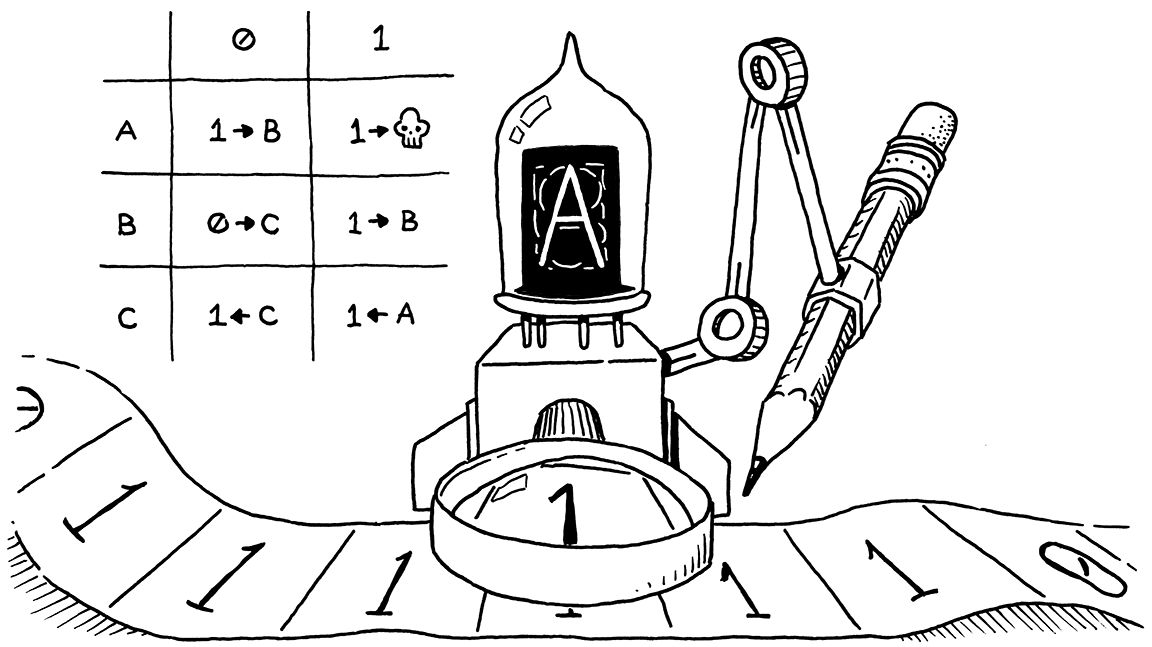
\includegraphics[width=.9\textwidth, keepaspectratio]{./pics/turing-machine-titlepage.png}
                \end{center}

                \vfill

                \par\noindent\rule{\textwidth}{0.8pt}
                \vspace*{0.6cm}
                \large
                \emph{Anno Accademico 2021-2022}

        \end{center}
\end{titlepage}


\setstretch{1.35}

%\title{Complessità}
%\author{Marco Sgobino}
%\maketitle
\tableofcontents

%\part{Complessità}
\chapter{La macchina di Turing}
\section{Descrizione}
TODO rifai tutti i disegni presi dall'insegnante.

Una \emph{macchina di Turing} è una macchina che è descritta da un insieme di
\emph{simboli} $\Gamma = \{\alpha, \beta, \gamma, \delta, \dots\}$ \emph{finito} e da
un insieme di \emph{stati} $\mathcal{Q} = \{q_1, q_2, \dots, q_n\}$ anch'esso
\emph{finito}. La macchina di Turing dispone di un nastro di memoria \emph{potenzialmente
illimitato} a destra e a sinistra; essa è in grado di identificare il simbolo
nella posizione dove la \emph{testina} della macchina è collocata sul nastro.
Ad ogni iterazione della macchina di Turing, viene letto il simbolo
ove sia collocata la sua testina; a seconda dello stato $q_i$, viene intrapresa
un'azione, che può essere una fra le $3$ seguenti:
\begin{itemize}
    \item spostamento della testina a destra;
    \item spostamento della testina a sinistra;
    \item riscrittura del simbolo sotto la testina con uno qualsiasi
        appartenente all'alfabeto di simboli.
\end{itemize}

Una macchina di Turing può anche essere accompagnato da un alfabeto
\emph{ausiliario}, ovverosia un alfabeto $\mathcal V$ comprendente simboli
simili a quelli di $\Gamma$, ma che vengono utilizzati qualora la macchina di
Turing avesse \emph{già processato} la cella in questione. Tipicamente,
l'utilizzo dell'alfabeto ausiliario è importante nel caso specifico in cui si
adoperino algoritmi e procedure per le quali è d'interesse ricordare se una
cella sia già stata in precedenza processata dalla macchina di Turing, oppure
no.

Nello specifico, una macchina di Turing è univocamente identificata dalla sua
\emph{matrice di transizione} $\delta  : \mathcal Q \times \Gamma \rightarrow
\mathcal Q \times (\Gamma \cup \{L,R\})$\footnote{In talune circostanze, è
possibile trovare una definizione differente, cioè $$\delta  : \mathcal Q \times
\Gamma \rightarrow \mathcal Q \times \Gamma \times \{L,R\};$$ in altre parole, è
una macchina che \emph{si muove sempre sul nastro,} poiché per ogni stato è
sempre definito un movimento. Per questo tipo di macchina, sono necessarie
diverse regole d'ingaggio, e i programmi in essa costruiti saranno radicalmente
differenti. La differenza fra i due modelli rappresenta un'evidenza della
versatilità della macchina di Turing.}, dove i simboli $L$ ed $R$ sono
rappresentativi dell'azione di spostarsi, rispettivamente, a sinistra e a
destra del nastro di memoria. La matrice di transizione lega, dunque, ciascuno
stato al simbolo collocato immediatamente sotto alla testina nel nastro di
memoria, stabilendo in maniera univoca l'azione da intraprendere. L'insieme
delle azioni che la macchina di Turing compie è quindi la realizzazione del
programma stesso.



\begin{table}[ht]
\centering
\begin{tabular}{c|cccc}
    & $q_1$ & $q_2$ & $\cdots$ & $q_n$ \\
    \hline
$\alpha$ & $\beta/q_2$ & $\gamma/q_2$ & $\cdots$ & \\
$\beta$ & $L/q_1$ & $\gamma/q_3$ & $\cdots$ & \\
$\gamma$ & $\gamma/q_3$ & $R/q_2$ & $\cdots$ & \\
$\vdots$ & $\vdots$ & $\vdots$ & $\ddots$ &    
\end{tabular}
\caption{Possibile matrice di transizione per una macchina di Turing. Le righe
corrispondono ai simboli dell'alfabeto $\Gamma$, mentre le colonne sono
corrispondenti ai singoli stati dell'insieme $\mathcal
Q$.}\label{tab:matriceTransizione}
\end{table}
\bigskip


Diversamente dal modello RAM, la quantità di memoria destinata ad ogni cella è
\emph{limitata}, poiché vi può essere collocato soltanto un numero finito di
simboli, quelli appunto dell'insieme $\Gamma$. Ciononostante, la macchina di
Turing si presta meglio alla trattazione di stringhe, poiché i simboli possono
rappresentare qualsivoglia tipologia di entità astratta, mentre per il modello
RAM si avrebbe necessità di una codifica fra numeri reali e simboli da
trattare: non vi è più dunque la limitazione imposta dal fatto che all'interno
di una cella possa risiedere esclusivamente un numero naturale, non importa
quanto grande sia; nella macchina di Turing le celle possono contenere simboli
di qualsiasi natura essi siano.

Tipicamente, all'alfabeto che definisce una macchina di Turing viene definito
un sottoinsieme sigma di simboli di input, $\Sigma \subset \Gamma$, in
concomitanza al quale viene definito un simbolo vuoto, \emph{blank}, $b \in
\Gamma - \Sigma$. Il simbolo $b$ rappresenta dunque l'idea di \emph{cella
vuota}. Ricapitolando, ogni macchina di Turing viene univocamente definita da:
\begin{itemize}
    \item un insieme finito di simboli $\Gamma$ \--- essi comprendono sia i
        simboli di input $\Sigma$ che il simbolo \emph{blank} $b$;
    \item un insieme finito di stati $\mathcal Q$;
    \item una funzione (matrice) di transizione $\delta  : \mathcal Q \times
        \Gamma \rightarrow \mathcal Q \times (\Gamma \cup \{L,R\})$.
\end{itemize}

Una diversa maniera per definire una macchina di Turing è tramite la
\emph{quaterna} o \emph{quadrupla} $q_i, s_j, \alpha, q_k$, dove $q_i$ è lo
\emph{stato in cui si trova la macchina}, $s_j$ è il \emph{simbolo letto dalla
testina}, $\alpha$ è il \emph{simbolo scritto nella matrice di transizione}, $q_k$ è
lo \emph{stato successivo} in cui la macchina di Turing si troverà al termine
dell'esecuzione di $\alpha$. In particolare, l'operazione che la macchina di
Turing effettua dipende dal simbolo $\alpha$ scritto nella matrice di
transizione:
\begin{itemize}
    \item se $\alpha = s_i$, sostituisci il simbolo $s_j$ con $s_i$;
    \item se $\alpha = R$, muovi la testina a destra;
    \item se $\alpha = L$, muovi la testina a sinistra;
\end{itemize}

Lo \emph{stop} della computazione di una macchina di Turing avviene qualora la
coppia $q_i, s_j$ \textbf{non} sia presente nella matrice di transizione.
Questa tecnica è analoga a quanto osservato per il modello RAM, nel quale la
macchina ha termine se si è giunti al termine della procedura e sono state
esaurite le istruzioni nella sequenza. Nel caso di una coppia simbolo\----stato
non presente nella matrice di transizione, la macchina di Turing si fermerà, e
vi sarà il riconoscimento del valore finale di computazione, espresso come nel
caso del modello RAM con una convenzione che permetta di identificare il valore
finale del risultato della computazione.

\section{Uso di una macchina di Turing}

Una macchina di Turing, come verrà illustrato in seguito, può essere espressa
anche mediante \emph{grafo} oltre che mediante matrice di sostituzione. In ogni
caso, ogni possibile definizione di macchina di Turing è del tutto equivalente,
e varia esclusivamente nella forma nella quale è proposta. Una macchina di
Turing, non importa come sia stata definita, può essere adoperata
sostanzialmente per compiere $3$ diversi operazioni:
\begin{enumerate}
    \item per il \emph{calcolo} di una funzione \--- la macchina di Turing è
        intesa come \emph{calcolatore}, e lo scopo è quello di calcolare una
        funzione $f: \mathbb{N}^n \rightarrow \mathbb{N}$. In questo caso, la
        macchina di Turing risulta essere meno efficiente del modello RAM, per
        via dell'assenza del comodo sistema di istruzioni presente in quest
        ultimo;
    \item per il \emph{riconoscimento} di una stringa \--- la macchina di
        Turing è intesa come \emph{accettore}. In questo contesto la MdT è
        molto più efficiente del modello RAM, poiché non è richiesta la
        codifica da numeri naturali a simboli;
    \item per la \emph{decisione} di un predicato \--- la macchina di Turing è
        intesa come \emph{decisore}.
\end{enumerate}

Convenzionalmente, l'esito di una macchina di Turing è una particolare
configurazione di memoria dello stato finale. In particolare, si è scelto che
il risultato $f(x)$ sia da leggersi come il numero totale di occorrenze di $1$
(meno una) sul nastro nella configurazione iniziale, se la computazione è
andata a convergenza \-- indefinito altrimenti. La sequenza di occorrenze del
simbolo $1$ è delimitata dal carattere \emph{blank}. Per quanto invece riguarda
i risultati di tipo \emph{vettoriale}, cioè del tipo $f(x_1,x_2,\dots,x_n)$,
ebbene sarà sufficiente costruire $n$ ``quadrati'' in cui racchiudere gli $x+1$
simboli $1$, ciascuno delimitato dal simbolo \emph{b}. In altre parole, la
situazione è quella descritta dalla Figura~\ref{fig:mdtRisultato}.

TODO figura mdtRisultato

Solitamente, è particolarmente difficile programmare sulla macchina di
Turing~\--~questo è principalmente dovuto al fatto che la macchina di Turing è
una macchina a stati, dove non vi è un insieme di istruzioni da applicare
direttamente, ma bisogna determinare la matrice di transizione relativa a ciò
che bisogna calcolare, stato per stato e simbolo per simbolo.


\section{Equivalenza fra macchina di Turing e $\mathcal R$}

Un importante teorema definisce l'equivalenza della macchina di Turing (avente
insieme delle funzioni computabili $\mathcal{TC}$ all'insieme delle funzioni
parziali ricorsive $\mathcal R$, e lo lega indissolubilmente all'insieme delle
funzioni computabili dal modello RAM $\mathcal C$.

\begin{thm}{dell'equivalenza della macchina di Turing all'insieme $\mathcal R$}
    $$\mathcal R \equiv \mathcal {TC} \equiv \mathcal C$$
\end{thm}

Un possibile spunto di dimostrazione di $\mathcal {TC} \subseteq \mathcal R$ si
ha per il fatto che la configurazione e lo stato della MdT durante la
computazione possono essere codificati da un numero naturale; le operazioni
sulla macchina sono rappresentate da funzioni ricorsive su questi numeri. Il
viceversa è invece mostrabile tenendo conto che si può verificare che
$\mathcal{TC}$ contiene le funzioni di base ed è chiusa rispetto a sostituzione,
ricorsione e minimazione illimitata.

\section{Potenziamento apparente della macchina di Turing}

Una macchina di Turing può essere potenziata mediante l'estensione di essa
tramite l'uso di \emph{nastri multitraccia}. In altre parole, anziché adoperare
un singolo nastro, si adoperano più nastri contemporaneamente. La macchina di
Turing viene espansa tramite l'aggiunta di uno \emph{stato della memoria
suppletiva}, che sostanzialmente ci indica il numero del nastro dove la
macchina di Turing sta agendo. Dunque, ci possiamo immaginare una macchina di
Turing con tanti nastri e tante testine che lavorano contemporaneamente, come
elencato in Figura~\ref{fig:macchina-turing-multinastro}.

\begin{figure}[b]
    \centering
    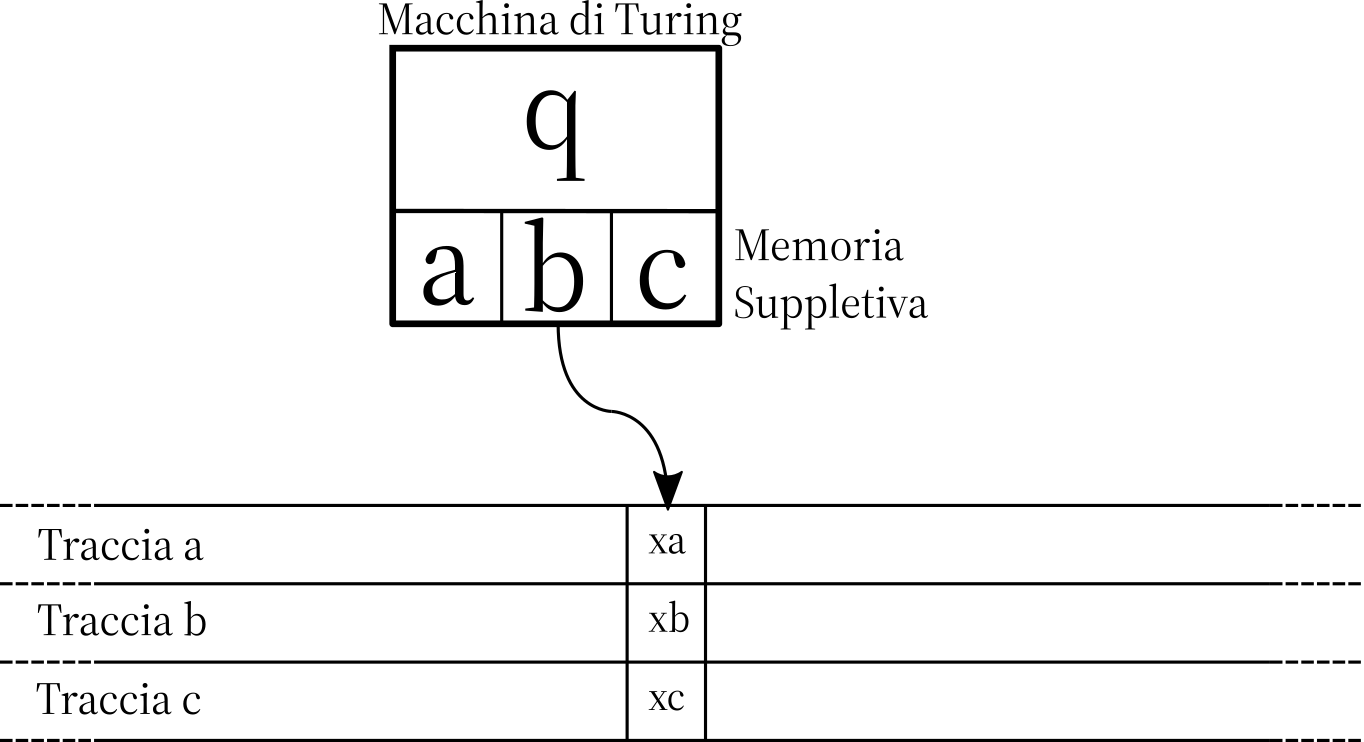
\includegraphics[ width=.8\linewidth, height=\textheight, keepaspectratio]{./pics/macchina-turing-multinastro.png}
    \caption{Macchina con memoria con nastro multitraccia.}
    \label{fig:macchina-turing-multinastro}
\end{figure}

Dal punto di vista della capacità computazione, una macchina di Turing
multinastro non aumenta né diminuisce le capacità \-- tuttavia, tale
rappresentazione può avere il vantaggio di presentare una maggiore somiglianza
con il tipo di computazione svolto all'interno di un computer moderno. Si pensi
infatti alla memoria RAM, alla memoria cache, al disco rigido e così via; una
macchina di Turing può dunque ``simulare'' qualsiasi computer
moderno\footnote{Un computer può a sua volta simulare da una macchina di
Turing, dal momento che possono essere applicati potenzialmente infiniti banchi
di memoria al computer \-- nella pratica, tuttavia, sappiamo che ciò non è
possibile, e i banchi di memoria non saranno mai del tutto \emph{illmitati}}.

Una macchina di Turing multinastro deve essere implementata con un
\emph{sistema multitraccia} \-- in altre parole, vengono adoperate \emph{tante
testine quante sono i nastri}. Ci si può facilmente ricondurre alla macchina di
Turing convenzionale semplicemente eliminando il sistema multitraccia, o per
meglio dire, una macchina di Turing multitraccia può essere \emph{simulata} da
una macchina di Turing convenzionale: essa dunque, non produce alcun tipo di
miglioramento dal punto di vista computazione, cioè le due macchine hanno la
\emph{stessa} potenza computazionale
(Figura~\ref{fig:mdt-equivalenza-multitraccia}. 

Il medesimo discorso si applica anche al tentativo di \emph{menomare} la
macchina di Turing, nel senso che potremmo pensare di rendere il nastro
semi-infinito, cioè illimitato solo a destra o solo a sinistra
(Figura~\ref{fig:macchina-turing-riduzione}). In tal caso, tuttavia, benché
questa apparente limitazione venga messa in atto, di fatto la macchina di
Turing menomata avrà la medesima capacità computazionale di quella
``standard'', perché possiamo sempre avere a disposizione una quantità
illimitata di memoria, o far uso di trucchi come quello dell'alfabeto
ausiliario $\mathcal V$.
\begin{figure}[b]
    \centering
    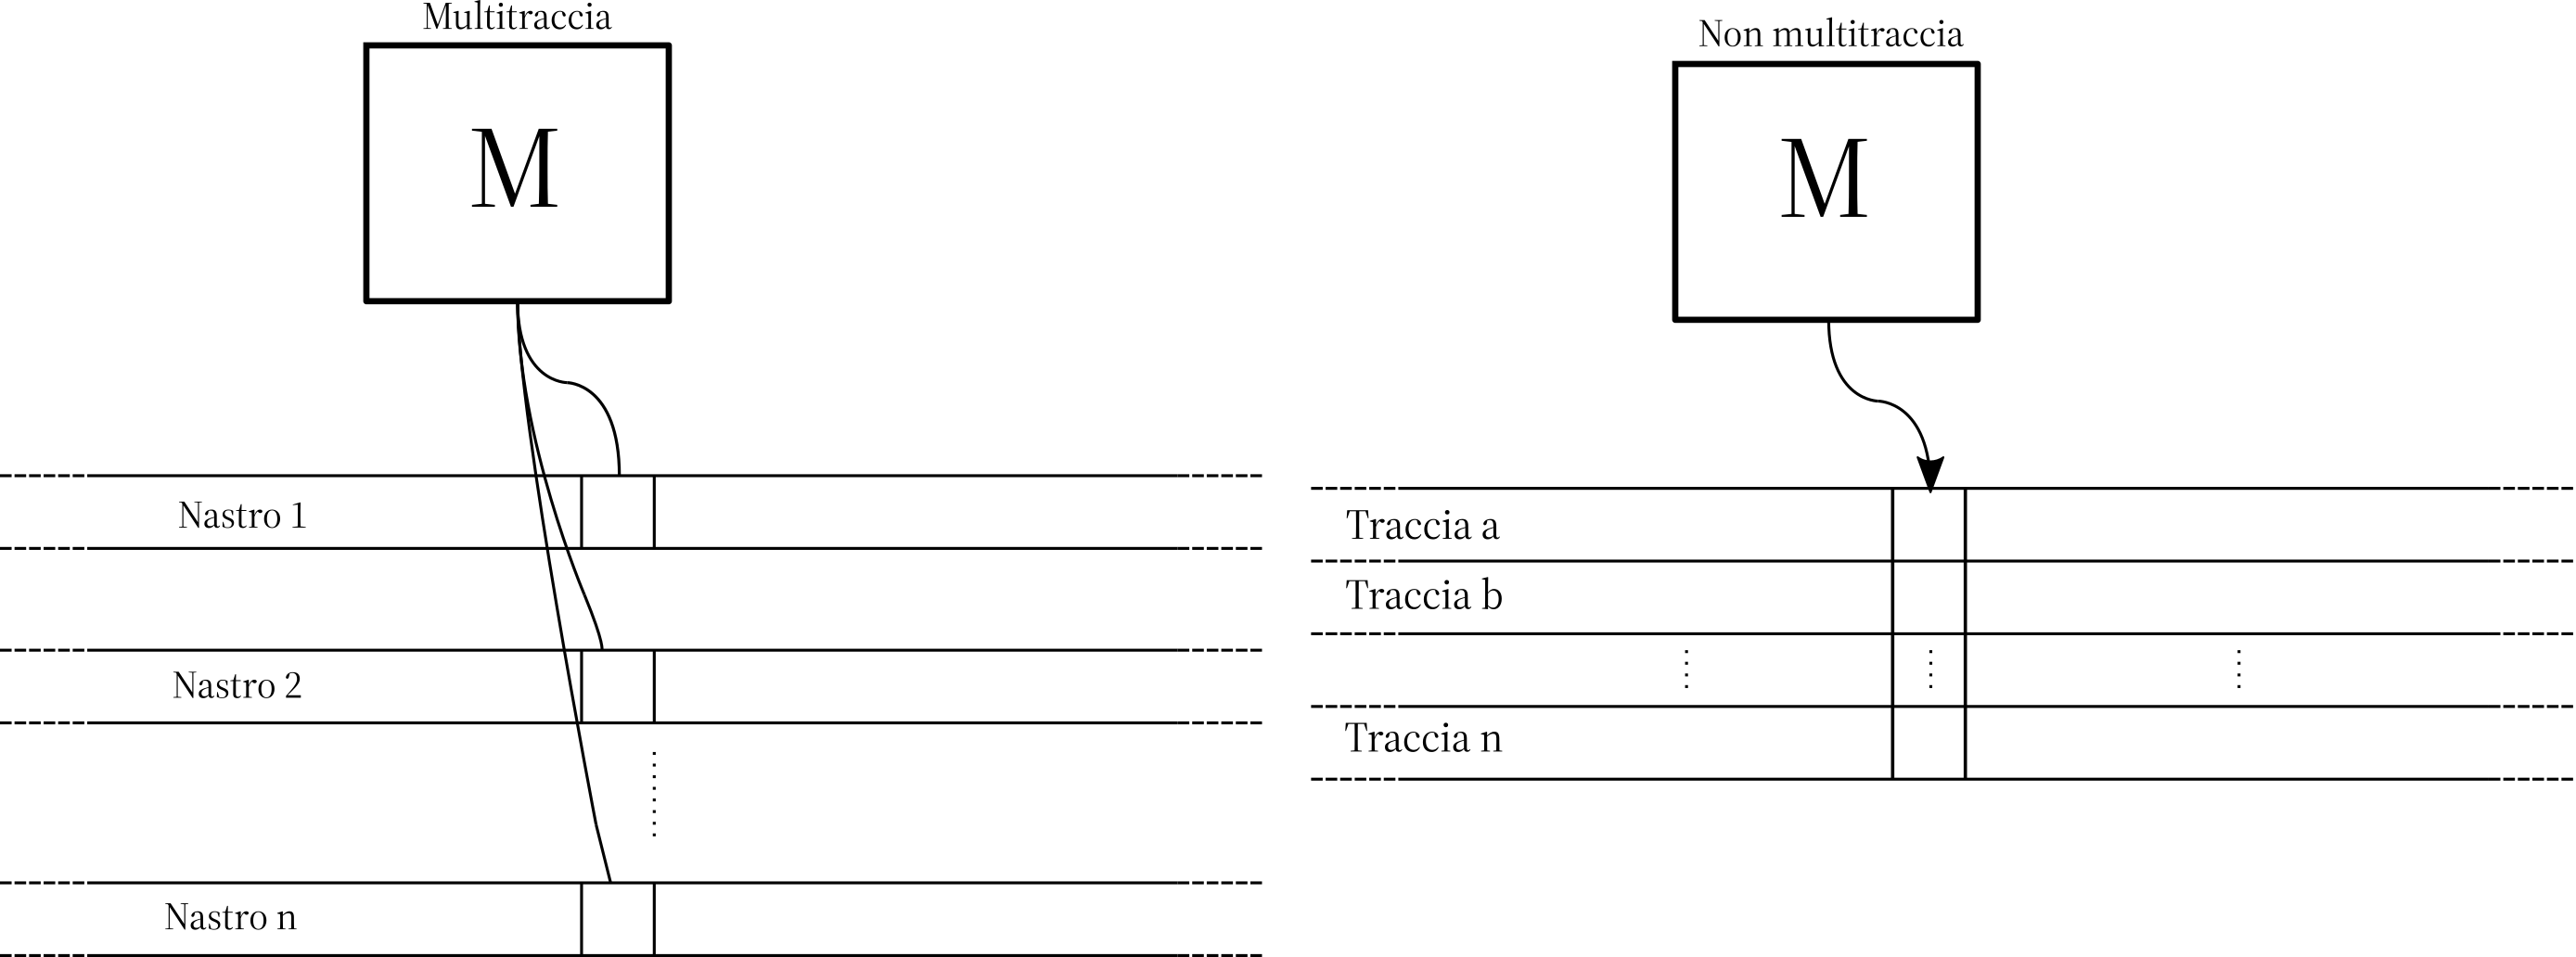
\includegraphics[ width=1.2\linewidth, height=\textheight, keepaspectratio]{./pics/mdt-equivalenza-multitraccia.png}
    \caption{Equivalenza fra una macchina di Turing a multitraccia e una
    macchina di Turing a singola testina.}
    \label{fig:mdt-equivalenza-multitraccia}
\end{figure}

\begin{figure}[b]
    \centering
    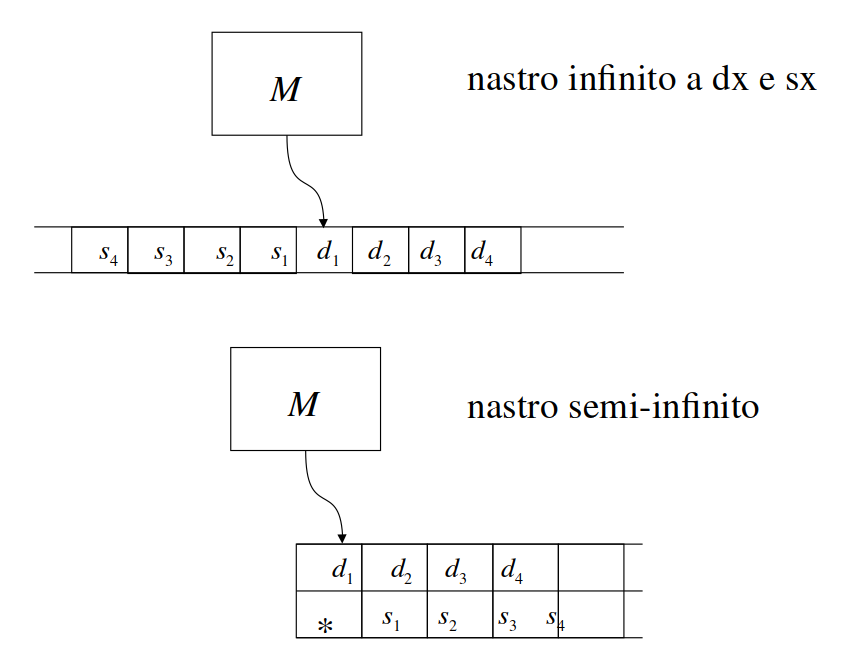
\includegraphics[ width=.7\linewidth, height=\textheight, keepaspectratio]{./pics/macchina-turing-riduzione.png}
    \caption{Equivalenza fra macchina di Turing a nastro illimitato solo a
    destra e a nastro illimitato da ambedue le parti.}
    \label{fig:macchina-turing-riduzione}
\end{figure}

\clearpage


\section{Macchina RAM per \emph{accettare} stringhe}

Nel modello RAM, per accettare una stringa è necessario operare una codifica.
In particolare, la stringa viene codificata in un numero naturale e la macchina
risponde con ``1'' o ``0'' a seconda che la stringa venga o meno accettata. Con
la macchina di Turing, invece, si può far intervenire direttamente uno
\emph{stato di accettazione} \textsc{Accettazione} $q_Y$ o uno \emph{stato di
rifiuto} \textsc{Rifiuto} $q_N$. Un'altra possibilità è quella di semi-decidere
riguardo l'accettazione di una stringa, cioè una macchina in grado di
riconoscere la stringa in questione, ma di non poter rifiutare la stringa,
poiché ci sarebbe un'infinita computazione, e dunque divergenza. Tipicamente,
lo stato iniziale viene denotato con $q_0$, e potrebbero esserci degli stati
ulteriori ``intermedi''. Un esempio di accettazione è dato dalla macchina
illustrata in Figura~\ref{fig:mdtAccettazione1}. La macchina riconosce il
linguaggio dato dalle stringhe con due ``zeri'' nelle ultime due posizioni a
destra, in particolare tutte le stringhe che terminano con ``00''.

\begin{figure}[b]
    \centering
    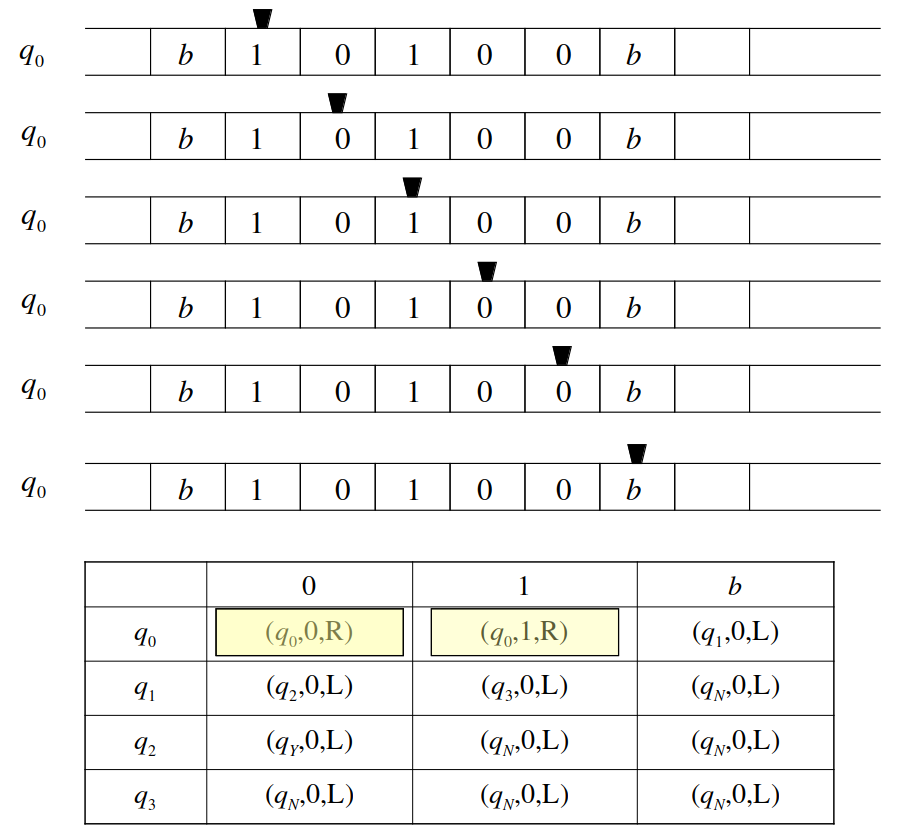
\includegraphics[ width=1.0\linewidth, height=\textheight, keepaspectratio]{./pics/mdtAccettazione1.png}
    \caption{Macchina che riconosce il linguaggio dato dalle stringhe con due $0$
nelle ultime due posizioni a destra, e suo funzionamento.}
    \label{fig:mdtAccettazione1}
\end{figure}

TODO aggiungi mdt definita a grafo

Una macchina di Turing può anche essere ``definita a grafo''. In questo modello
di definizione, la macchina di Turing,
\begin{itemize}
    \item ha un \emph{nastro semi-illimitato} a destra, diviso in celle;
    \item ha un alfabeto \emph{ausiliario} $\mathcal V$;
    \item ha un simbolo di spaziatura $\Delta$, equivalente al simbolo
        \emph{blank} $b$;
    \item un puntatore, del tutto equivalente alla testina;
    \item un \emph{programma}, definito come \textbf{grafo finito orientato},
        con i vertici definiti come \emph{stato}. Vi è uno stato di inizio,
        indicato con \textsc{Inizio}, e un sottoinsieme eventualmente vuoto di
        stati di arresto, indicati con \textsc{Accettazione}. I nodi del grafo
        sono collegati da \emph{archi}.
\end{itemize}

Ciascun arco è della forma

TODO rifai
\begin{verbatim}
(i) ---(alpha, beta, gamma) ---> (j)
\end{verbatim}

dove $$\alpha \in \Sigma \cup \mathcal V \cup \{\Delta\}, \beta \in \Sigma \cup
\mathcal V \cup \{\Delta\} \mbox{ e } \gamma \in \{L, R\}.$$ Dunque, siamo
nello stato $i$; la macchina legge $\alpha$, scrive $\beta$ al posto di
$\alpha$, e infine va a destra oppure a sinistra a seconda che il simbolo
$\gamma$ sia pari ad $R$ o ad $L$.

TODO aggiungi esempio lettura stringa speciale

Tale problema espresso qui sopra (add figure) è molto noto nella teoria della
computabilità, poiché è un tipico esempio di problema che è risolubile da una
macchina di Turing, ma \textbf{non risolubile} mediante una macchina \emph{a
stati finiti}. Le macchine a stati finiti, infatti, non presentano alcun tipo
di \emph{memoria}, e dunque per questa particolare mancanza non sono in grado
di risolvere il problema. La macchina di Turing, invece, è in grado di
risolverlo in virtù della sua superiore potenza di computazione.


\chapter{Le macchine non deterministiche}

Oltre alla macchina di Turing, sono possibili altre tipologie di macchine, con
vari livelli di gerarchia fra potenze di calcolo. Il seguente elenco ne
illustra alcune,

\begin{itemize}
    \item macchine a \emph{stati finiti}: in questo caso, hanno $0$
        \emph{memorie push-down} \-- le macchine a stati finiti sono le meno
        potenti in assoluto dal punto di vista computazionale, e non sono in
        grado di risolvere il problema TODO add figure del riconoscimento di
        stringhe $a^n b^n$;
    \item macchine a \emph{$1$ memoria push-down}: dotata di una memoria
        push-down, ha una maggiore potenza di calcolo rispetto alla macchina a
        stati finiti;
    \item macchine a \emph{$2$ memorie push-down}: dotata di $2$ memorie
        push-down, essa è equivalente alla macchina di Turing.
    \item una macchina con $3$ o più pile push-down non fornisce vantaggi dal
        livello della potenza computazionale, e sono tutte Turing-equivalenti
        \-- il vantaggio è semmai nella semplificazione di calcoli fornita
        dall'introduzione della pila aggiuntiva.
\end{itemize}


\section{Alcune definizioni sulle stringhe}

Sia dato l'alfabeto $\Sigma^*$. Faremo uso di tre fondamentali funzioni
definite su $\Sigma^*$:
\begin{itemize}
    \item l'operazione $testa(x)$, che fornisce la ``testa'' di una stringa,
        ovverosia la lettera di estrema sinistra della parola $x$;
    \item l'operazione $coda(x)$, la quale invece fornisce la ``coda'' di una
        stringa, o la stringa privata della sua testa $x$;
    \item l'operazione $\sigma \cdot x$, che \emph{concatena} la lettera
        $\sigma$ e la parola $x$, per formare un'unica parola nuova.
\end{itemize}


\section{Gerarchie delle potenze di calcolo}

La gerarchia delle potenze di calcolo è la seguente, dall'alto verso il basso:
\begin{enumerate}
    \item Macchine non deterministiche di Turing, con due memorie
        push-down~\----~Macchine di Turing, Modello RAM, Macchine di Post,
        macchine finite con due memorie push-down (sono in grado di accettare
        $\{a^n b^n a^n| n \geq 0\}$). Si potrebbe dimostrare che le macchine di
        Turing deterministiche e non deterministiche hanno la medesima potenza
        di calcolo; 
    \item Macchine finite non deterministiche con una memoria push-down, sono
        in grado di riconoscere $\{w w^R | w\in\{a,b\}^*\}$\footnote{Il
        \emph{nodo di decisione} che introduce il non determinismo serve per
    gestire la situazione data dall'incapacità di riconoscere il punto di
rottura $ww^R$, cioè il punto in cui finisce $w$ ed inizia $w^R$. Con il non
determinismo, ogniqualvolta si arriva al nodo di decisione si tengono valide
entrambe le possibilità \-- dunque, è più potente.};
    \item macchine finite con una memoria push-down, riconoscono $\{a^n
        b^n|n\geq 0\}$;
    \item Macchine finite non deterministiche senza memorie push-down \----
        macchine finite senza memorie push-down \---- automi finiti.
\end{enumerate}

\section{La macchina di Turing non deterministica}

La macchina di Turing effettiva è di tipo \emph{deterministico}. Il \emph{non determinismo} viene introdotto per due ragioni:
\begin{itemize}
    \item si desidera osservare se una macchina di Turing non deterministica
        sia o meno più \emph{potente} di una macchina di Turing deterministica;
    \item si cerca di valutare se possano esistere differenti paradigmi di
        computazione (ad esempio, computazione parallela).
\end{itemize}

Una \emph{macchina di Turing non deterministica} può avere nel suo diagramma di flusso dei \emph{nodi di decisione} del tipo seguente, TODO add figure

ovverosia dei nodi dove a fronte di un medesimo simbolo vi sono \emph{più archi
possibili} \-- il non determinismo viene dunque introdotto da questo fenomeno:
una macchina di Turing non deterministica può scegliere il suo percorso con una
legge non deterministica, ma semmai dettata dal caso o da una \emph{scelta
arbitraria}. Una macchina non deterministica accetta l'idea che vi siano più
possibilità di sviluppo di una computazione a fronte di un medesimo simbolo
identificato sul nastro e stato; sono dunque possibili diversi percorsi di
computazione. Questo tipo di macchina, ad esempio, potrebbe concepire il
\emph{parallelismo} nella computazione, nel senso che più possibilità e
percorsi nel calcolo sono possibili. Questa potenzialità, apparentemente
migliorativa, \textbf{non aumenta} la potenza di calcolo della macchina di
Turing. Una macchina di Turing deterministica può, infatti, simulare una
macchina non deterministica, è sufficiente compiere una ricerca per ogni
diramazione dell'albero dei nodi \-- con un aumento esponenziale del numero di
operazioni da effettuare, ma pur sempre realizzabile e computabile da una
macchina di Turing. Una macchina non deterministica ha dunque il potenziale
vantaggio di poter risolvere problemi in \emph{tempo lineare} che dalla
macchinia deterministica sarebbero risolti in in tempo esponenziale.

In questo caso, il parallelismo è insito nella macchina non deterministica, e
la stringa si considera \emph{accettata} qualora uno qualunque fra i percorsi
possibili incappa nello stato di \textsc{Accettazione}. Una parola $w \in
\Sigma^*$ si dice \emph{accettata} da una macchina di Turing non deterministica se
esiste una computazione della macchina $M$ che cominci con entrata $x=w$, e che
termini ad un arresto con lo stato di \textsc{Accettazione}. Se $w$ non viene
accettata e lo stato di arresto è quello del \textsc{Rifiuto}, allora si dice
che $w$ è \emph{rifiutata}. In alternativa, siamo di fronte ad un ciclo $w \in
ciclo(M)$.

In altre parole, possiamo pensare ad una macchina di Turing non deterministica
come ad un macchina avente per ogni cella, nella matrice di transizione, un
\emph{insieme} $\delta(q,s)$ di triple $q_i, s_i, \alpha_i$, dove $\alpha_i \in
\{L,R\}$ e ad ogni elemento dell'insieme corrisponde una possibile scelta da
compiere arbitrariamente o casualmente, e dunque da lì è ottenuto il non
determinismo della macchina. Ogni possibile scelta genererà un diverso ramo
nell'albero della computazione \-- per l'accettazione di un simbolo è
sufficiente che uno \emph{qualsiasi} fra i rami di computazione termini nello
stato di \textsc{Accettazione}. Dunque, benché una macchina di Turing non
deterministica non \textbf{aumenti} la potenza di calcolo intrinseca della
macchina, essa consente la \textbf{parallelizzazione} dei possibili percorsi
della computazione, rendendo di fatto possibile risolvere in tempo lineare
problemi che sarebbero risolubili (comunque), ma in tempo esponenziale per una
macchina deterministica.

\subsection{Equivalenza fra macchine non deterministiche e macchine multinastro}

\begin{thm}
    Ogni macchina di Turing non deterministica ha un equivalente macchina di
    Turing deterministica multinastro.
\end{thm}

\textsc{Dimostrazione} \---- Una traccia della dimostrazione è una ricerca
nell'albero di computazione. Con almeno due nastri, si simula con uno la
macchina non deterministica mentre con l'altro si collezionano tutti i
possibili $k$ ``prossimi passi'' della tabella di transizione. La macchina di
Turing deterministica allora controllerà tutte le configurazioni
stato\----simbolo, livello per livello, dell'albero di computazione. Lo stato
finale di \textsc{Accettazione} terminerà la computazione complessiva.

L'idea è quella, dunque, di \emph{simulare} il non determinismo compiendo un
numero crescente in modo esponenziale di passi, uno per ogni ramo dell'albero
non deterministico di computazione.

\begin{thm}
    Ogni macchina di Turing non deterministica $T_M(n)$ ha un equivalente
    macchina di Turing deterministica con ordine $2^{O(T_M(n))}$.
\end{thm}

\textsc{Dimostrazione} \---- Una traccia può essere che il numero massimo di
foglie è $O(b^{T_M(n)})$, dove $b$ è il numero di figli. Il tempo per viaggiare
dalla radice lungo ogni ramo è, per una macchina multinastro,
$$O(T_M(n)b^{T_M(n)}) = 2^{O(T_M(n))},$$ mentre per una macchina a nastro
singolo $$(2^{O(T_M(n))})^2 = 2^{O(2T_M(n))} = 2^{O(T_M(n))},$$ dunque l'ordine
è lo stesso.

In altre parole, una macchina non deterministica è in grado di ``evocare'' un
numero esponenziale ed arbitrariamente elevato di macchine di Turing
deterministiche \-- tale funzionalità però è irrealizzabile, poiché
corrisponderebbe a dotare la propria macchina di un numero arbitrario di unità
di calcolo, ciascuna per ogni possibile passo della computazione, per farle
lavorare in parallelo.


\chapter{Le reti neuronali di Hopfield}

Le \emph{reti neuronali} incarnano un diverso paradigma rispetto a quello della
computazione procedurale. Storicamente, esse prendono spunto dalla natura, in
particolare dal concetto di \emph{neurone}, inteso come singola unità di
calcolo, dotata di input, di output e di una \emph{funzione caratteristica}.
Diversamente dall'idea della computazione procedurale, dove la
\emph{complessità} è definita tramite la complessità di tipo computazionale (o
temporale), le reti neuronali esprimono la loro complessità attraverso la
\textbf{complessità strutturale}, o \textbf{complessità circuitale}. La
computazione è di tipo \emph{collettivo}, ed emerge come proprietà
dell'\emph{evoluzione dinamica} della rete. Ogni decisore locale, detto
\emph{neurone}, non ha visibilità della computazione globale, e svolge il
proprio compito localmente \---- ogni decisore locale concorre alla soluzione
globale in modo sfumato: la rete è \textbf{robusta} rispetto a malfunzionamenti
locali.

Dal punto di vista strettamente logico, il paradigma di computazione a reti
neuronali è l'unico paradigma radicalmente differente da quello procedurale,
mentre il paradigma \emph{a DNA}\footnote{Trattasi di un paradigma di calcolo
dove si va a cercare lo spazio delle soluzioni, e si eleggono quelle più
``performanti'' \---- talune soluzioni saranno la base dalla quale saranno
definite le successive soluzioni, convergendo dunque alla soluzione. La potenza
di questo metodo è quello di potersi permettere una ricerca esauriente della
soluzione, poiché ciascun DNA è infinitesimamente piccolo, e dunque può essere
esaminato in parallelo.} è una tipologia di calcolo che, nella realtà, non
differisce sostanzialmente dal metodo procedurale.

Esistono due filoni di reti neuronali; il primo associato ai
\textbf{perceptron}, macchine a strati che fungono da riconoscitori di pattern
e configurazioni. Le variabili di ingresso rappresentano un ente, una
configurazione del sistema esterno, e il perceptron è in grado di fornire in
output una risposta che consente di riconoscere tale configurazione o pattern
in base a come essa sia stata configurata e ai suoi parametri. Il secondo
filone, invece, è quello della \emph{rete di Hopfield}; tale filone sarebbe in
grado, in linea di principio, di \textbf{risolvere problemi}. Mediante una
rete di Hopfield è possibile risolvere il \emph{travelling salesman problem},
un problema presumibilmente intrattabile\footnote{``Presumibilmente'' si
riferisce al fatto che, fino ad ora, nessuno è riuscito a dimostrare né che
tale problema può essere risolto in tempo polinomiale, né che non può esserlo}.

Le reti neuronali hanno avuto grande successo in $3$ periodi storici:
\begin{itemize}
    \item all'inizio degli anni $40$ \-- nel $1948$ fu fornito il primo modello
        di neurone e rete neuronale. L'idea fu quella di avvalersi di una
        macchina fisica per simulare il comportamento dei neuroni naturali,
        presenti nel nostro cervello. All'epoca uscirono anche articoli su
        memorie a breve e lungo termine adoperando reti neuronali;
    \item durante gli anni $80$ \-- nei primi anni $80$, Hopfield individuò un
        modello di reti neuronali che associava le reti neuronali ad un
        particolare modello matematico; qualità che prima era assente. Si
        tratta di una caratteristica fondamentale: quando si cerca di risolvere
        problemi con le reti neuronali, l'assenza di teoremi (ad esempio,
        quelli asintotici) non ci permette di stabilire la \emph{qualità} di
        una soluzione, oppure se la computazione andrà in qualche maniera a
        buon fine. Dunque, l'assenza di un buon apparato matematico che faccia
        da base alle reti neuronali è il principale svantaggio di tale
        paradigma. Hopfield riuscì a fornire la soluzione di alcuni fra questi
        problemi matematici, suggerendo la possibilità di risolvere problemi,
        come ad esempio quello sopra citato del \emph{travelling salesman
        problem}. Ci fu allora una corsa dal punto di vista scientifico
        riguardo la possibilità di risolvere in maniera efficiente i problemi
        presumibilmente intrattabili. Si può dimostrare, tuttavia, che la
        potenza di computazione di una macchina di Hopfield \textbf{non è
        superiore} alla capacità di computazione della macchina di Turing. Con
        una macchina di Hopfield non è dunque possibile risolvere in tempo
        polinomiale problemi che non sono risolubili in tale maniera già dalla
        macchina di Turing \-- vi è dunque l'\emph{equivalenza} fra le due
        macchine. Le reti di Hopfield caddero pertanto ben presto in disuso;
    \item il terzo ed ultimo periodo d'oro delle reti neuronali è al giorno
        d'oggi, dove la potenza di calcolo superiore delle macchine moderne
        apre la strada ad un uso maggiormente ampio delle reti neuronali, che
        si avvalgono della pura potenza computazionale di gran lunga maggiore
        rispetto al passato per produrre risultati in tempo apprezzabile.
\end{itemize}

\section{Il neurone reale ed il neurone simulato}

Una macchina di Hopfield simula un neurone reale. Vi sono all'incirca $10^{11}$
neuroni (dieci miliardi) nel cervello, i quali formano una rete neuronale di
una complessità disarmante. Il cervello è in grado di svolgere una quantità di
compiti enorme, in modo efficiente \-- il cervello dunque è la struttura più
complessa che esista nell'universo noto. I segnali elettrici nel cervello si
sviluppano nell'ambito dei \emph{segnali continui} (benché vi siano degli
\emph{spike}), tuttavia il suo funzionamento si svolge nell'ambito dei
\emph{segnali discreti}; un neurone si ``eccita'' o si ``rilassa'',
manifestando dunque un comportamento del tutto discreto da questo punto di
vista.

TODO aggiungi figure neuroni, hopfield, e tutto il resto




\end{document}
